
\begin{lemma}{Mitternachtsformel}
    $x=\frac{-b\pm\sqrt{b^2-4ac}}{2a}$
\end{lemma}

\begin{theorem}{Polynomdivision} \emph{!} Vorzeichen von Nullstellen umdrehen\\
    $\frac{P(x)}{q(x)} = S(x) + \frac{r(x)}{q(x)}$ \qquad $P,q,S,r$ Polynome
\end{theorem}


\raggedcolumns
\paragraph{Funktionen}
\small

\begin{definition}
    {Komposition/Verkettung} $(g \circ f)(x)=g(f(x))$
\end{definition}


\begin{definition}{Stetigkeit} \small
    Funktion ist stetig, falls Kurve keine Sprünge macht und man Graphen der Funktion zeichnen kann, ohne Stift abzusetzen.
\end{definition}

\begin{definition}{Gleichmässige Konvergenz}
    $\forall x$ Linksseitiger Grenzwert = Rechtsseitiger GW
\end{definition}

\begin{concept}{Symmetrie} gerade $f(-x)=f(x)$, ungerade $f(-x)=-f(x)$
\end{concept}

\begin{KR}{Trick Ungerade Funktionen}
    $\int_{-a}^{+a} f(x) \dif x = 0$
    \begin{itemize}
        \item Summe/Komposition: ungerade und ungerade $\rightarrow$ ungerade
        \item Produkt/Quotient: ungerade und gerade $\rightarrow$ ungerade
        \item Ableitung: gerade $\longrightarrow$ ungerade
    \end{itemize}
    Ungerade: $f(x)$ = $-x$, $x$, $sin(x)$, $tan(x)$, Polynomfunkt. (ungerader Exponent)\\
    Gerade: $1$, $x^2$, $cos(x)$, $sec(x)$, Polynomfunkt. mit geradem Exponent\\
    Gerade und Ungerade: $f(x) = 0$, $f(x) = C$ (Konstante)
\end{KR}


\paragraph{Trigonometrische Funktionen}
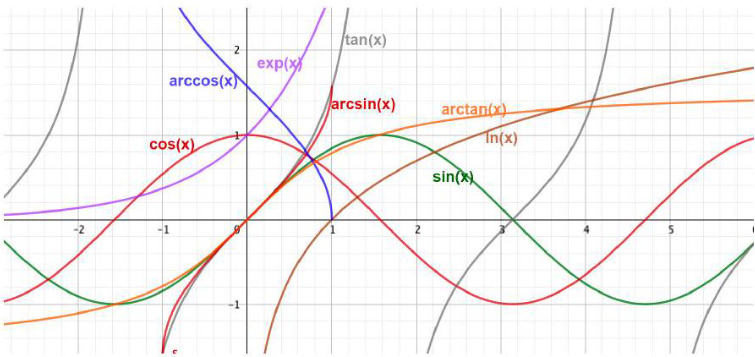
\includegraphics[width=0.8\linewidth]{trigonometrische_funktionen.png}
\begin{remark}
    $\tan x = \frac{\sin x}{\cos x}$ und $\cot x = \frac{\cos x}{\sin x}$ 
\end{remark}


\begin{corollary}{Eigenschaften sin/cos} \small
    \begin{itemize}
        \item $\cos x = \cos(-x) ~\text{und}~ \sin(-x) = -\sin x$
        \item $\sin(x + y) = \sin(x)\cos(y) + \cos(x)\sin(y)$
        \item $\cos(x + y) = \cos(x)\cos(y) - \sin(x)\sin(y)$
        \item $\sin^2(x) = \frac{1 - \cos(2x)}{2} \quad \cos^2(x) = \frac{1 + \cos(2x)}{2}$ $\rightarrow$ $\cos^2(x) + \sin^2(x) = 1$
        \item $\sin(2x) = 2 \sin(x)\cos(x)$ \hspace{4mm} $\cos(2x) = \cos^2(x) - \sin^2(x)$
         \item $\sin(x + \frac{\pi}{2}) = \cos(x), \quad \cos(x + \frac{\pi}{2}) = -\sin(x)$
         \item $\sin(x+\pi) = -\sin (x), \quad \sin(x + 2\pi) = \sin(x)$
         \item $\cos(x+\pi) = -\cos (x), \quad \cos(x + 2\pi) = \cos(x)$
     \end{itemize}
 \end{corollary}

 \begin{KR}{Nullstellen von trigonometrischen Funktionen}
    \begin{enumerate}
         \item $\text{Nullstellen Sinus} = \{k\cdot \pi : k\in \mathbb{Z}\}$ \\
        $\sin(x) > 0 \quad \forall x \in ]2k\pi, ~(2k+1)\pi[, ~ k\in \mathbb{Z}$\\[2pt]
        $\sin(x) < 0 \quad \forall x \in ](2k + 1)\pi, ~(2k+2)\pi[, ~ k\in \mathbb{Z}$\\
        $\pi$: kleinste strikt positive Nullstelle von $\sin$
        \item $\text{Nullstellen Cosinus} = \left\{\frac{\pi}{2}+k\cdot \pi : k\in \mathbb{Z}\right\}$\\
        $\cos(x) > 0:\forall x \in \left]-\frac{\pi}{2} +2k\pi, ~-\frac{\pi}{2} +(2k+1)\pi\right[, ~ k\in \mathbb{Z}$\\[2pt]
        $\cos(x) < 0:\forall x \in \left]-\frac{\pi}{2} + (2k + 1)\pi, ~-\frac{\pi}{2} +(2k+2)\pi\right[, ~ k\in \mathbb{Z}$
    \end{enumerate}
\end{KR}
 
\begin{concept}{Rechnen mit Logarithmen} $log_b (a) = \frac{ln(a)}{ln(b)}$
    \small
    \begin{itemize}
        \item $\ln (a \cdot b) = \ln a + \ln b \quad \forall a,b \in ]0 +  \infty[$
        \item $\ln (a \div b) = \ln a - \ln b \quad \forall a,b \in ]0 +  \infty[$
        \item ${\ln (x^a) = a \ln (x) \quad \forall a \in \R, \forall x > 0}$
    \end{itemize} 
\end{concept}


\raggedcolumns








\subsubsection{Integralrechnung}

\begin{concept}{Integralregeln} $(\lambda_1,\lambda_2 \in \mathbb{R} )$
    \begin{itemize}
      \item Addition/Subtraktion:
      $\int f(x-k) d x=F(x-k)+C$
      \item Multiplikation:
      $\int f(x \cdot k) d x=\frac{1}{k} F(x \cdot k)+C$
      \item Skalarmultiplikation:
      $\int \lambda_{1} f(x)+\lambda_{2} g(x) d x=\lambda_{1} F(x)+\lambda_{2} G(x)+C$
      \item Linearkombination: $\int{(\lambda_1f(x)+\lambda_2g(x))} = \lambda_2F(x)+\lambda_2G(x)+C$
      \item Verschiebung um k in x-Richt.: $\int{f(x-k)\mathrm{d}x}= F(x-k)+C$
      \item Streckung um k in x-R.: $\int{f(k\cdot x)\mathrm{d}x}= \frac{1}{k}F(k\cdot x)+C (k\neq0 )$
    \end{itemize}
\end{concept}


\begin{theorem}{Partielle Integration}

	$\int_a^b f(x) g'(x) \dif x = f(b) g(b) - f(a) g(a) - \int_a^b f'(x)g(x) \dif x$
   
   Unbestimmte:
   $
   \int(f(x) \cdot g^{\prime}(x)) d x=f(x) \cdot g(x)-\int(f^{\prime}(x) \cdot g(x)) d x
   $
\end{theorem}




\begin{theorem}{Substitution}
    $\int_{g(b)}^{g(a)} f(x) \dif x = \int_{a}^b f(g(t)) g'(t) \dif t$
    \vspace{1mm}\\
   Unbestimmte Integrale: $\int f(g(t)) \cdot g^{\prime}(t) d t=\left.\int f(x) d x\right|_{x=g(t)}$
\end{theorem}

\begin{corollary}{Nützliche Regeln}
	Sei $I \subseteq \R$ ein Intervall und $f: I \to \R$ stetig.
    
    $\int_{a+c}^{b+c} f(x) \dif x = \int_{a}^{b} f(t+c) \dif t$ und $\int_{a}^{b} f(ct) \dif t = \frac{1}{c} \int_{ac}^{bc} f(x) \dif x$
\end{corollary}

\begin{KR}{Substitution}
    $u=g(x),\quad \frac{\mathrm{d}u}{\mathrm{d}x}=g'(x),\quad \mathrm{d}x = \frac{\mathrm{d}u}{g'(x)} $
    \begin{itemize}
	\item Durchführen der Substitution \(u=g(x) \)	 und \(\mathrm{d}x=\frac{\mathrm{d}u}{g'(x)} \):\\
	    $\int{f(x)\mathrm{d}x}=\int{r(u)}{\mathrm{d}u} \text{ bzw. } \int_a^b{f(x)\mathrm{d}x}=\int_{g(a)}^{g(b)}{r(u)}{\mathrm{d}u}$
	\item Berechnen des Integrals mit Variable u:\\
	    $\int{r(u)\mathrm{d}u}=R(u)+C \text{ bzw. } \int_{g(a)}^{g(b)}{r(u)\mathrm{d}u}=R(u)+C\Big|_{g(a)}^{g(b)}$
	\item Rücksubstitution:\\
	    $R(u)+C=R(g(x))+C$ bzw. $R(u)+C\Big|_{g(a)}^{g(b)}=R(g(x))+C\Big|_{g(a)}^{g(b)}$
    \end{itemize}	
\end{KR}


\begin{example2}{Nützliche Substitutionen}
    \begin{itemize}
        \item $\log (x)$ subst: $t=\log (x), x=e^{t}, d x=e^{t} d t$
        \item für gerade $n: \cos ^{n}(x), \sin ^{n}(x), \tan (x)$ \\Sub: $t=\tan (x)$, $d y=\frac{1}{1+t^{2}} d t, \sin ^{2}(x)=\frac{t^{2}}{1+t^{2}}, \cos ^{2}(x)=\frac{1}{1+t^{2}}$
        \item für ungerade $n: \cos ^{n}(x), \sin ^{n}(x)$, \\Sub: $t=\tan (x / 2)$, $d y=\frac{2}{1+t^{2}} d t, \sin (x)=\frac{2 t}{1+t^{2}}, \cos (x)=\frac{1-t^{2}}{1+t^{2}}$
        \item $\int \sqrt{1-x^{2}} d x$ sub: $x=\sin (x)$ oder $\cos (x)$
        \item $\int \sqrt{1+x^{2}} d x$ sub: $x=\sinh (x)$
    \end{itemize}
\end{example2}

\begin{concept}{Uneigentliche Integrale}
\begin{itemize}
    \item $I=\int_a^{\infty}{f(x)\mathrm{d}x}=\underset{\lambda \rightarrow \infty}{\lim}I(\lambda)=
		\underset{\lambda \rightarrow \infty}{\lim}(\int_a^{\lambda}{f(x)\mathrm{d}x})$
    \item $I=\int_{-\infty}^{\infty}{f(x)\mathrm{d}x}=\int_{-\infty}^{c}{f(x)\mathrm{d}x}+\int_c^{\infty}
		{f(x)\mathrm{d}x} = \underset{\lambda \rightarrow -\infty}{\lim}I(\lambda)+$
    \item $I=\int_a^b{f(x)\mathrm{d}x}=\underset{\epsilon \rightarrow 0}{\lim}I(\epsilon)=\underset{\epsilon \rightarrow
	0}{\lim}(\int_{a+\epsilon}^b{f(x)\mathrm{d}x})$
\end{itemize}
\end{concept}

\begin{KR}{Flächeninhalt zwischen zwei Kurven $f(x)$ und $g(x)$}
		$$\left|\int_{a}^{x_{1}}(f(x)-g(x)) d x\right|+\left|\int_{x_{1}}^{x_{2}}(f(x)-g(x))\right|+\cdots+\left|\int_{x_{n}}^{b}(f(x)-g(x))\right|$$
\end{KR}


\begin{theorem}{Mittelwert einer Funktion}
    $\mu = \frac{1}{b-a}\int_a^b{f(x)\mathrm{d}x}$

    \small
    $\rightarrow$ Höhe des Rechtecks mit $l$ = $b-a$ und Flächeninhalt $A = \int_a^b{f(x)\mathrm{d}x}$.
\end{theorem}

\begin{corollary}{Wichtige Integrale}
    \begin{itemize}
        \item Rotationsvolumen: $V = \pi \int_a^b{(f(x))^2\mathrm{d}x} $
        \item Bogenlänge: $L = \int_a^b{\sqrt{1+(f'(x))^2}\mathrm{d}x} $
        \item Mantelfläche: $M = 2\pi \int_a^b{f(x)\cdot \sqrt{1+(f'(x))^2}\mathrm{d}x}$
    \end{itemize}
\end{corollary}




\raggedcolumns





    \resizebox*{\linewidth}{!}{
	\def\arraystretch{1.7}
	\begin{tabular}{c|c|c}
	    Ableitung | f'(x)                          & Funktion | f(x)                          & Integral | F(x)                       \\
        \hline
	    \(0\)                                      & \(C\)                                    & \(x+C\)                               \\
        \hline
        \(1\)                                      & \(x\)                                    & \(\frac{1}{2}x^2+C\)                  \\
        \hline
        \(-\frac{1}{x^2}\)                         & \(\frac{1}{x}\)                          & \(\ln|x|+C\)                          \\
        \hline
        \(ax^{a-1}\)                               & \(x^a \: with \: a \: \in \: \mathbb{R}\) & \(\frac{x^{a+1}}{a+1}+C\)             \\
        \hline
        $x^{x} \cdot(1+\ln x) \quad x>0$          & $x^{x}$                                  &   \\
        \hline        
        $\frac{1}{2\sqrt{x}}$                     & $\sqrt{x}$                               &  $\frac{2}{3}x^{\frac{3}{2}}$         \\
        \hline
        $\frac{1}{n} x^{\frac{1}{n}-1}$           & $\sqrt[n]{x}$                            & $\frac{n}{n+1} x^{\frac{1}{n}+1}$     \\
        \hline
        \(\ln(a)\cdot a^x\)                       & \(a^x\)                                  & \(\frac{a^x}{\ln(a)}+C\)              \\
        \hline
        $a^{b x} \cdot c \ln a$                   & $a^{b x}$                                & $\frac{1}{b \ln a} a^{b x}$             \\
        \hline
        \(e^x\)                                   & \(e^x\)                                  & \(e^x+C\)                             \\
        \hline
        \(\frac{1}{x}\)                           & \(\ln(x)\)                               & \(x\ln(x)-x+C\)                       \\
        \hline
        \(\frac{1}{x\ln(a)}\)                     & \(\log_a(x)\)                            & \(x\log_a(x)-\frac{x}{\ln(a)}+C\)     \\
        \hline
        \(\cos(x)\)                                & \(\sin(x)\)                              & \(-\cos(x)+C\)                        \\
        \hline
        \(-\sin(x)\)                               & \(\cos(x)\)                              & \(\sin(x)+C\)                         \\
        \hline
        \(1+\tan^2{(x)=\frac{1}{\cos^2{(x)}}}\)    & \(\tan(x)\)                              & \(-\ln|\cos(x)|+C\)                   \\
        \hline
        \(-1-\cot^2{(x)}=-\frac{1}{\sin^2{(x)}}\)  & \(\cot(x)\)                              & \(\ln(\sin(x))+C\)                    \\
        \hline
        \(\frac{1}{\sqrt{1-x^2}}\)                & \(\arcsin(x)\)                           & \(x\arcsin(x)+\sqrt{1-x^2}+C\)        \\
        \hline
        \(-\frac{1}{\sqrt{1-x^2}}\)               & \(\arccos(x)\)                           & \(x\arccos(x)-\sqrt{1-x^2}+C\)        \\
        \hline
        \(\frac{1}{1+x^2}\)                       & \(\arctan(x)\)                           & \(x\arctan(x)-\frac{1}{2}\ln(1+x^2)+C\)\\
        %add more here
        \hline
        $\sin ^{2}(x)$                            & $\frac{1}{2}(x-\sin (x) \cos (x))$       & $\sin (x) \cos (x) + C$                   \\
        \hline
        $\cos ^{2}(x)$                            & $\frac{1}{2}(x+\sin (x) \cos (x))$       & $\cos (x) \sin (x) + C$                   \\ 
        \hline
        $\tan ^{2}(x)$                            & $\tan (x)-x$                             & $\tan (x) + C$                            \\
        \hline
        $\cot ^{2}(x)$                            & $-\cot (x)-x$                            & $\cot (x) + C$                            \\
        \hline
        $\frac{f'(x)}{f(x)}$                      & $\ln |f(x)|$                             & $x \cdot(\ln |x|-1) + C$                 \\
        \hline
        $\frac{-f^{\prime}(x)}{(f(x))^{2}}$       & $\frac{1}{f(x)}$                         & \\
        \hline
        $(a x+b)^{n}$                             & $\frac{1}{a \cdot(n+1)}(a x+b)^{n+1}$   & \\
        \hline
	\end{tabular}
    }



\subsubsection{Differentialrechnung}

\begin{concept}{Ableitungsregeln}
    Seien $f,g: D \to \R$  differenzierbar. Dann gelten:
    \begin{itemize}
        \item Summe/Differenz: $(f + g)'(x) = f'(x) + g'(x)$
        \item Faktor: $f(x)=a\cdot g(x) \rightarrow f'(x)=a \cdot g'(x) $
        \item Produkt: $(f \cdot g)'(x) = f'(x)g(x) + f(x)g'(x)$
        \item Quotient: $(\frac{f}{g})'(x) = \frac{f'(x) g(x) - f(x) g'(x)}{g(x)^2}$
        \item Kettenregel: $(g \circ f)' (x) = g'(f(x)) f'(x)$
        \item Umkehrfunktion: $(f^{-1})'(y_0) = \frac{1}{f'(x)}$
        \item Potenz/Logarithmus 1: 
        $(a^{f(x)})' = ln(a) \cdot a^{f(x)} \cdot f'(x)$

        \resizebox{\linewidth}{!}{
            $(f(x)^{g(x)})' = f(x)^{g(x)} \cdot (ln(f(x)) \cdot g(x))' =  f(x)^{g(x)} \cdot (ln(f(x)) \cdot g(x) \cdot \frac{f'(x)}{f(x)})$
            }
    \end{itemize}
\end{concept}

\begin{theorem}{Sekanten-Steigung/Differentialquotient}
    $\frac{\Delta f}{\Delta \mathrm{x}}=\frac{f(x_{0}+h)-f(x_{0})}{h}$
\end{theorem}

\begin{comment}
\begin{corollary}{Krümmung}
    Zusammenhang zwischen 2. Ableitung und Krümmung:
    \begin{itemize}
      \item $f^{\prime \prime}(x_{0})>0$ Konvex (Nach links/oben gekrümmt)
      \item $f^{\prime \prime}(x_{0})<0$ Konkav (Nach rechts/unten gekrümmt)
      \item $f^{\prime \prime}(x_{0})=0$ Keine eindeutige Krümmung
    \end{itemize}
    Bmk: Die Summe zweier konvexer Funktionen ist konvex. (konkav analog)
\end{corollary}
\end{comment}

\begin{corollary}{Kurvendiskussion} $f(x) = y$
    \begin{itemize}
        \item $f'(x) = 0$ $ \Rightarrow$ $x$ lokales Extremum (NST)
        \item Bestimme $f''(x)$ (Zweite Ableitung)
		\begin{itemize}
			\item $f''(x) = 0$ $ \Rightarrow$ siehe Vorgehen Wende- und Sattelpunkte
			\item $f''(x) < 0$ $ \Rightarrow$ relatives Maximum
			\item $f''(x) > 0$ $ \Rightarrow$ relatives Minimum
		\end{itemize}
    \end{itemize}
    Vorgehen Wende- und Sattelpunkte:
    \begin{itemize}
        \item Wendepunkt: $f^{(3)}(x_{0}) \neq 0$ 
        \item Sattelpunkt: zusätzlich $f^{\prime}(x_{0})=0$ 
    \end{itemize}
    Punkt bestimmen: In Gleichung $f(x) = y$ einsetzen $\rightarrow$ $P(x, y)$
\end{corollary}















































